\documentclass[10pt,twocolumn]{article}

\usepackage{graphicx}
\usepackage[colorlinks=true,allcolors=blue]{hyperref}

\begin{document}

\title{Next-generation design tools for intelligent transportation systems}
\author{Dominik Ascher and Georg Hackenberg}
\maketitle

\begin{abstract}
    TODO
\end{abstract}

\section{Introduction}
\label{sec:introduction}

TODO~\cite{ascher_hackenberg_2014,ascher_hackenberg_2015,ascher_hackenberg_2016,ascher_hackenberg_2017}

\subsection{Research objective}

With our research, we want to help improve the efficiency and effectiveness of today's transportation systems.
To achieve this goal, we work on methodologies for designing such systems and verifying their properties.
Fundamentally, we promote a formal approach capturing the relevant design decisions and their relations.
Furthermore, we integrate scenario-based simulation of system dynamics and evaluation of emergent properties.
Finally, we exploit optimization algorithms for optimizing system dynamics as well as static design decisions.

\subsection{Research question}

In this paper, we ask how the next generation of design tools for intelligent transportation systems should look like.
Therefore, first we want to understand which system properties and design decisions should be represented in these tools.
Then, we want to learn how the design decisions could be verified with respect to the desired system properties.
Finally, we want to study how the relevant design information could be represented in a graphical user interface.

\subsection{Research methodology}

In the following, we first propose a modeling and simulation framework for capturing design decisions and evaluating emergent properties in Section~\ref{sec:framework}.
Then, we propose a graphical user interface for building system designs, starting simulation runs, and visualizing simulation outcomes in Section~\ref{sec:gui}.
Thereafter, we propose two special applications of our modeling and simulation framework as well as user interface technology in Section~\ref{sec:application}.
Finally, we draw our conclusions and describe future direction of research and development on the design of ITS in Section~\ref{sec:conclusion}. 

\section{Underlying framework}
\label{sec:framework}

In this section, we propose a modeling and simulation framework for the design of intelligent transportation systems.
We first introduce a modeling technique for describing the design decisions and defining evaluation scenarios in Section~\ref{sec:modeling-technique}.
Then, we propose an interface for implementing and integrating custom control strategies in Section~\ref{sec:controller-interface}.
Finally, we define an interface for collecting statistics during simulation of system dynamics in Section~\ref{sec:statistics-interface}.

\subsection{Modeling technique}
\label{sec:modeling-technique}

TODO

\begin{figure*}[tbp]
    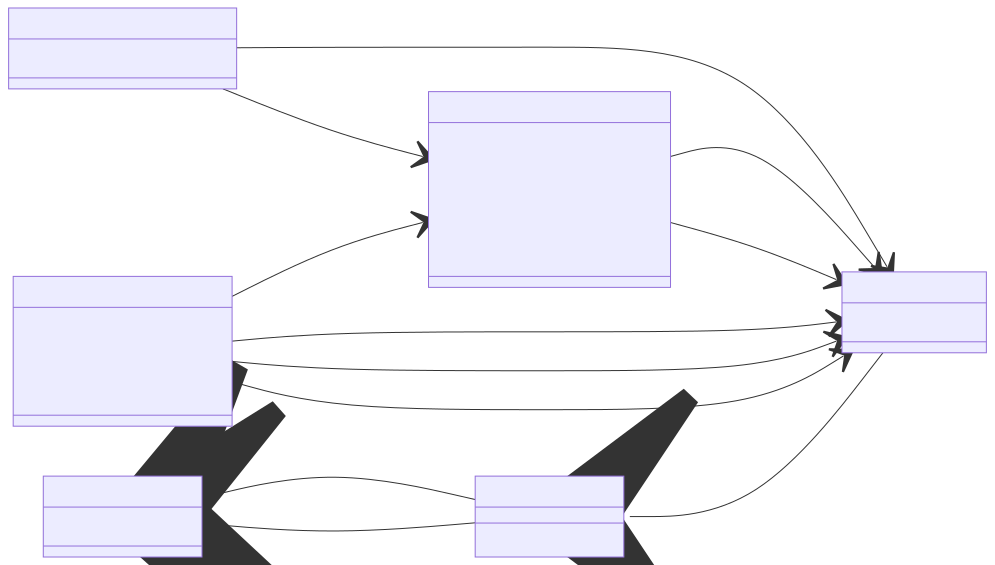
\includegraphics[width=\textwidth]{../../diagrams/model/classes-v0.1.png}
    \caption{Modeling technique}
    \label{fig:modeling-technique}
\end{figure*}

TODO

\subsection{Controller interface}
\label{sec:controller-interface}

TODO

\begin{figure*}[tbp]
    \includegraphics[width=\textwidth]{../../diagrams/controller/classes.png}
    \caption{Controller interface}
    \label{fig:controller-interface}
\end{figure*}

TODO

\subsubsection{Manual controller}

TODO

\subsubsection{Random controller}

TODO

\subsubsection{Greedy controller}

TODO

\subsubsection{Smart controller}

TODO

\subsubsection{Switchable controller}

TODO

\subsection{Statistics interface}
\label{sec:statistics-interface}

TODO

\begin{figure}[htbp]
    \includegraphics[width=\columnwidth]{../../diagrams/statistics/classes.png}
    \caption{Statistics interface}
    \label{fig:statistics-interface}
\end{figure}

TODO

\section{Graphical user interface}
\label{sec:gui}

TODO

\begin{figure*}[tbp]
    \includegraphics[width=\textwidth]{../../screenshots/basic-simulation.png}
    \caption{Graphical user interface}
    \label{fig:gui}
\end{figure*}

TODO

\subsection{Map}

TODO

\subsection{Vehicle charts}

TODO

\subsubsection{Vehicle battery chart}

TODO

\subsubsection{Vehicle distance chart}

TODO

\subsection{Demand charts}

TODO

\subsubsection{Demand time chart}

TODO

\subsubsection{Demand distance chart}

TODO

\subsection{Infrastructure charts}

TODO

\subsubsection{Intersection chart}

TODO

\subsubsection{Segment chart}

TODO

\subsubsection{Station chart}

TODO

\section{Specific applications}
\label{sec:application}

TODO

\subsection{Controller comparison}
\label{sec:controller-comparison}

TODO

\begin{figure*}[tbp]
    \includegraphics[width=\textwidth]{../../screenshots/controller-comparison.png}
    \caption{Controller comparison}
    \label{fig:controller-comparison}
\end{figure*}

TODO

\subsection{Infrastructure comparison}
\label{sec:infrastructure-comparison}

TODO

\begin{figure*}[tbp]
    \includegraphics[width=\textwidth]{../../screenshots/infrastructure-comparison.png}
    \caption{Infrastructure comparison}
    \label{fig:infratructure-comparison}
\end{figure*}

TODO

\section{Conclusion}
\label{sec:conclusion}

TODO

\bibliographystyle{plain}
\bibliography{main}

\end{document}